\documentclass[conference]{IEEEtran}

\usepackage{graphicx}
\usepackage{amsmath,amssymb}
\usepackage{booktabs}
\usepackage{multirow}
\usepackage{cite}
\usepackage{url}
\usepackage{xcolor}
\usepackage[hidelinks]{hyperref}
\usepackage[caption=false,font=footnotesize]{subfig}
\usepackage{xurl}
\usepackage{float}
\usepackage{placeins}
\usepackage{balance}

\newcommand{\method}{CLIP-linear}
\newcommand{\dataset}{MS COCOAI}

\title{Cross-Generator AI-Generated Image Detection with CNN and CLIP Features}

\author{
\IEEEauthorblockN{Xufeiyang Shi}
\IEEEauthorblockA{
ECE4880J Computer Vision Final Project\\
Shanghai Jiao Tong University\\
Shanghai, China
}
}

\begin{document}
\maketitle

\begin{abstract}
AI-generated image detectors often achieve high accuracy on images from
generators seen during training, but may fail when evaluated on unseen
generators. This project studies this cross-generator distribution shift on
MS COCOAI, a 2026 dataset containing real images and synthetic images from
modern generators including Stable Diffusion 3, SDXL, DALL-E 3, and
MidJourney v6. I compare a ResNet-18 detector trained from scratch with a
frozen CLIP ViT-B/32 image encoder followed by a linear classifier. With
single-generator ResNet training, unseen-generator performance is weak in both
directions: SD3 to MidJourney gives unseen AUC 0.5318 and MidJourney to SD3
gives unseen AUC 0.5482. Adding SDXL to SD3 training improves ResNet's
MidJourney unseen AUC to 0.6694. The CLIP-linear detector improves all three
protocols, reaching unseen AUC 0.9018 and F1 0.7096 for SD3+SDXL to
MidJourney. These results show that generator diversity and pretrained
visual-semantic features both improve robustness under generator shift.
\end{abstract}

\begin{IEEEkeywords}
AI-generated image detection, cross-generator generalization, ResNet, CLIP,
image classification
\end{IEEEkeywords}

\section{Introduction}

Modern text-to-image systems can generate realistic images with diverse styles
and semantics. This progress creates a practical need for detectors that can
distinguish real photographs from AI-generated images. A major challenge is
\emph{cross-generator generalization}: a detector trained on one generator may
learn generator-specific artifacts and fail on images from a different
generator.

This project evaluates that failure mode using MS COCOAI~\cite{roy2026mscocoai},
a recent dataset built from MS COCO images~\cite{lin2014coco} and synthetic
images generated by Stable Diffusion 3, Stable Diffusion 2.1, SDXL, DALL-E 3,
and MidJourney v6. The goal is not only to maximize seen-generator accuracy,
but to measure whether a detector remains reliable under generator shift.

The project makes three empirical comparisons. First, I train a ResNet-18
detector on one generator and test it bidirectionally across SD3 and
MidJourney v6. Second, I test whether adding another training generator
(SDXL) improves held-out MidJourney performance. Third, I repeat the same
protocols with a frozen CLIP image encoder~\cite{radford2021clip} and a
linear classifier. The main finding is that ResNet-18 learns useful seen-domain
signals but generalizes poorly, while CLIP-linear features substantially
improve unseen-generator AUC and F1.

\section{Related Work}

Convolutional neural networks such as ResNet~\cite{he2016resnet} remain strong
image-classification baselines because they learn hierarchical visual features
directly from the training data. However, when trained from scratch on a narrow
generator distribution, they can overfit to low-level artifacts such as
texture, compression, and generator-specific rendering patterns.

CLIP~\cite{radford2021clip} is pretrained on large-scale image-text pairs with
a contrastive objective, producing image embeddings that capture broad
visual-semantic structure. Because these features are learned from diverse
web-scale data rather than a single fake-image generator, they may provide a
more robust representation for AI-generated image detection under distribution
shift.

\section{Method}

\subsection{Problem Formulation}

Each image $\mathbf{x}$ has a binary label $y \in \{0,1\}$, where $0$ denotes
real and $1$ denotes AI-generated. Both detectors produce two scores, one for
``real'' and one for ``fake''. A softmax layer converts these scores into a
fake probability:
\begin{equation}
p_{\mathrm{fake}}(\mathbf{x})=
\frac{\exp(s_{\mathrm{fake}})}
{\exp(s_{\mathrm{real}})+\exp(s_{\mathrm{fake}})}.
\end{equation}
During training, the model is penalized when the probability assigned to the
correct class is low. This is the standard cross-entropy objective:
\begin{equation}
\mathcal{L}(\theta)=
-\frac{1}{N}\sum_{i=1}^{N}\log p_{y_i}(\mathbf{x}_i).
\end{equation}
Evaluation is performed on validation, seen-generator test, and
unseen-generator test splits. The most important metric is unseen-generator
performance.

\subsection{ResNet-18 Baseline}

The first detector is a ResNet-18 classifier trained from scratch. Its
calculation pipeline is:
\begin{equation}
\mathbf{x}
\rightarrow
\mathrm{ResNet18}_{\theta}(\mathbf{x})
\rightarrow
[s_{\mathrm{real}},s_{\mathrm{fake}}]
\rightarrow
p_{\mathrm{fake}}.
\end{equation}
Images are resized and cropped to $224 \times 224$. The original ImageNet
classification layer is replaced with a two-class real/fake head. All ResNet
parameters are updated during training, so the network must learn both the
image representation and the final decision boundary from the curated
real/fake data. This makes it a clean test of whether a CNN trained from zero
can learn generator-invariant fake-image evidence.

\subsection{Frozen CLIP Feature Detector}

The second detector uses a frozen CLIP ViT-B/32 image encoder. Its calculation
pipeline is:
\begin{equation}
\mathbf{x}
\rightarrow
g_{\phi}(\mathbf{x})
\rightarrow
\mathbf{z}
\rightarrow
\mathbf{W}\mathbf{z}+\mathbf{b}
\rightarrow
p_{\mathrm{fake}}.
\end{equation}
Here $g_{\phi}$ is the CLIP image encoder and is not updated. It outputs a
512-dimensional image embedding, which is normalized before classification:
\begin{equation}
\mathbf{z}=
\frac{g_{\phi}(\mathbf{x})}
{\|g_{\phi}(\mathbf{x})\|_2}.
\end{equation}
Only the linear head parameters $(\mathbf{W},\mathbf{b})$ are trained. This
separates representation learning from the downstream real/fake classifier.
The reason for using CLIP is that its image encoder was pretrained with
large-scale image-text contrastive learning. Instead of learning only local
texture artifacts from one generator, CLIP starts from a feature space that
already captures object identity, scene layout, style, and visual-semantic
regularities. This should make the final detector less dependent on artifacts
from a single synthetic generator.

\section{Experiments}

\subsection{Dataset and Protocols}

MS COCOAI contains 96,000 real and synthetic datapoints generated from MS COCO
captions and images. The experiments follow a staged logic:
\begin{itemize}
    \item \textbf{Step 1a: ResNet SD3 $\rightarrow$ MidJourney.} Train from
    scratch on SD3 fakes and test on unseen MidJourney v6 fakes.
    \item \textbf{Step 1b: ResNet MidJourney $\rightarrow$ SD3.} Reverse the
    direction to check whether the transfer failure is symmetric.
    \item \textbf{Step 2: ResNet SD3+SDXL $\rightarrow$ MidJourney.} Add a
    second training generator to test whether generator diversity improves
    generalization.
    \item \textbf{Step 3: CLIP-linear comparison.} Repeat the same three
    protocols with frozen CLIP features and a trainable linear head.
\end{itemize}
For the single-generator protocols, the curated split contains 14,000 training
images, 3,000 validation images, 15,000 seen-test images, and 15,000
unseen-test images. For the two-generator protocol, it contains 28,000
training images, 6,000 validation images, 30,000 seen-test images, and 15,000
unseen-test images.

\subsection{Implementation Details}

All experiments run on an RTX 5090 GPU. ResNet-18 uses batch size 128, learning
rate $10^{-4}$, weight decay $10^{-3}$, dropout 0.2, label smoothing 0.05, and
early stopping with patience 2. CLIP-linear uses OpenAI CLIP ViT-B/32, batch
size 256 for feature extraction, learning rate $10^{-3}$ for the linear head,
weight decay $10^{-4}$, and early stopping with patience 8. Metrics are
accuracy, F1, and ROC AUC. F1 and AUC are reported with fake as the positive
class.

\section{Results}

\subsection{Step 1 and Step 2: ResNet-Only Results}

The first question is whether a CNN trained from scratch can learn a general
fake-image detector. Step 1 tests this with a bidirectional single-generator
transfer experiment. In Step 1a, ResNet is trained on SD3 fakes and evaluated
on unseen MidJourney fakes. In Step 1b, the direction is reversed. These two
runs are important because a robust detector should transfer in both
directions, not only from one convenient source domain.

\begin{figure}[H]
    \centering
    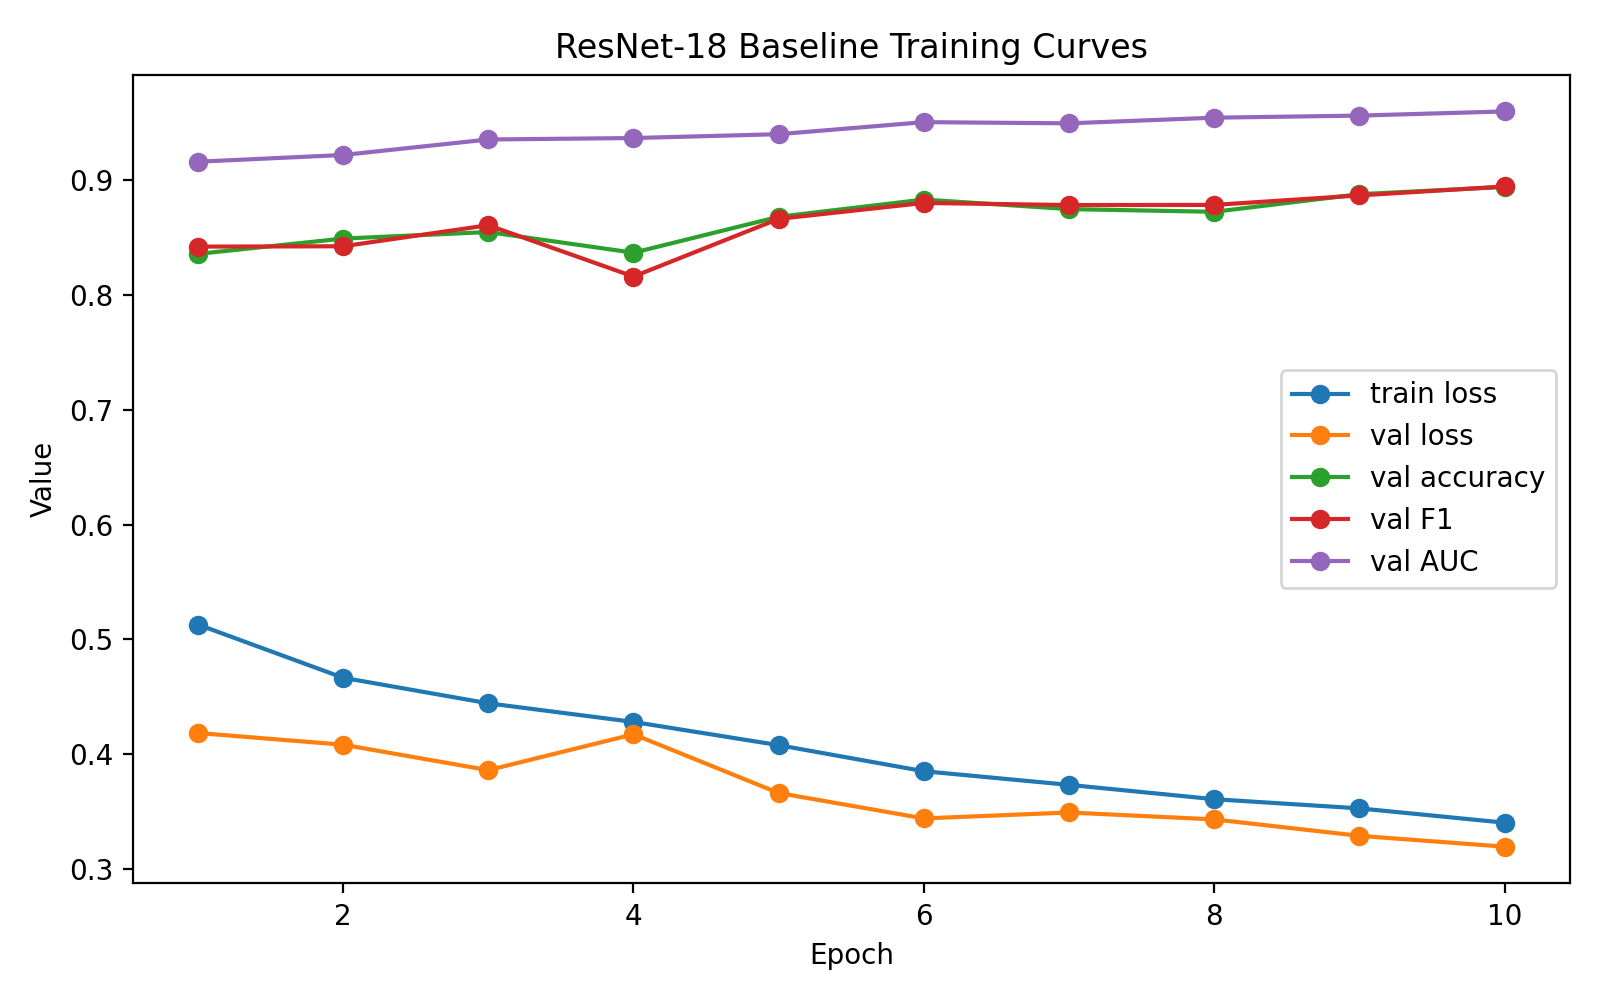
\includegraphics[width=0.95\columnwidth]{figures/step1a_resnet_training_curves.png}
    \caption{Step 1a ResNet training curves: SD3 $\rightarrow$ MidJourney.}
    \label{fig:step1a_resnet_curves}
\end{figure}

\begin{figure}[H]
    \centering
    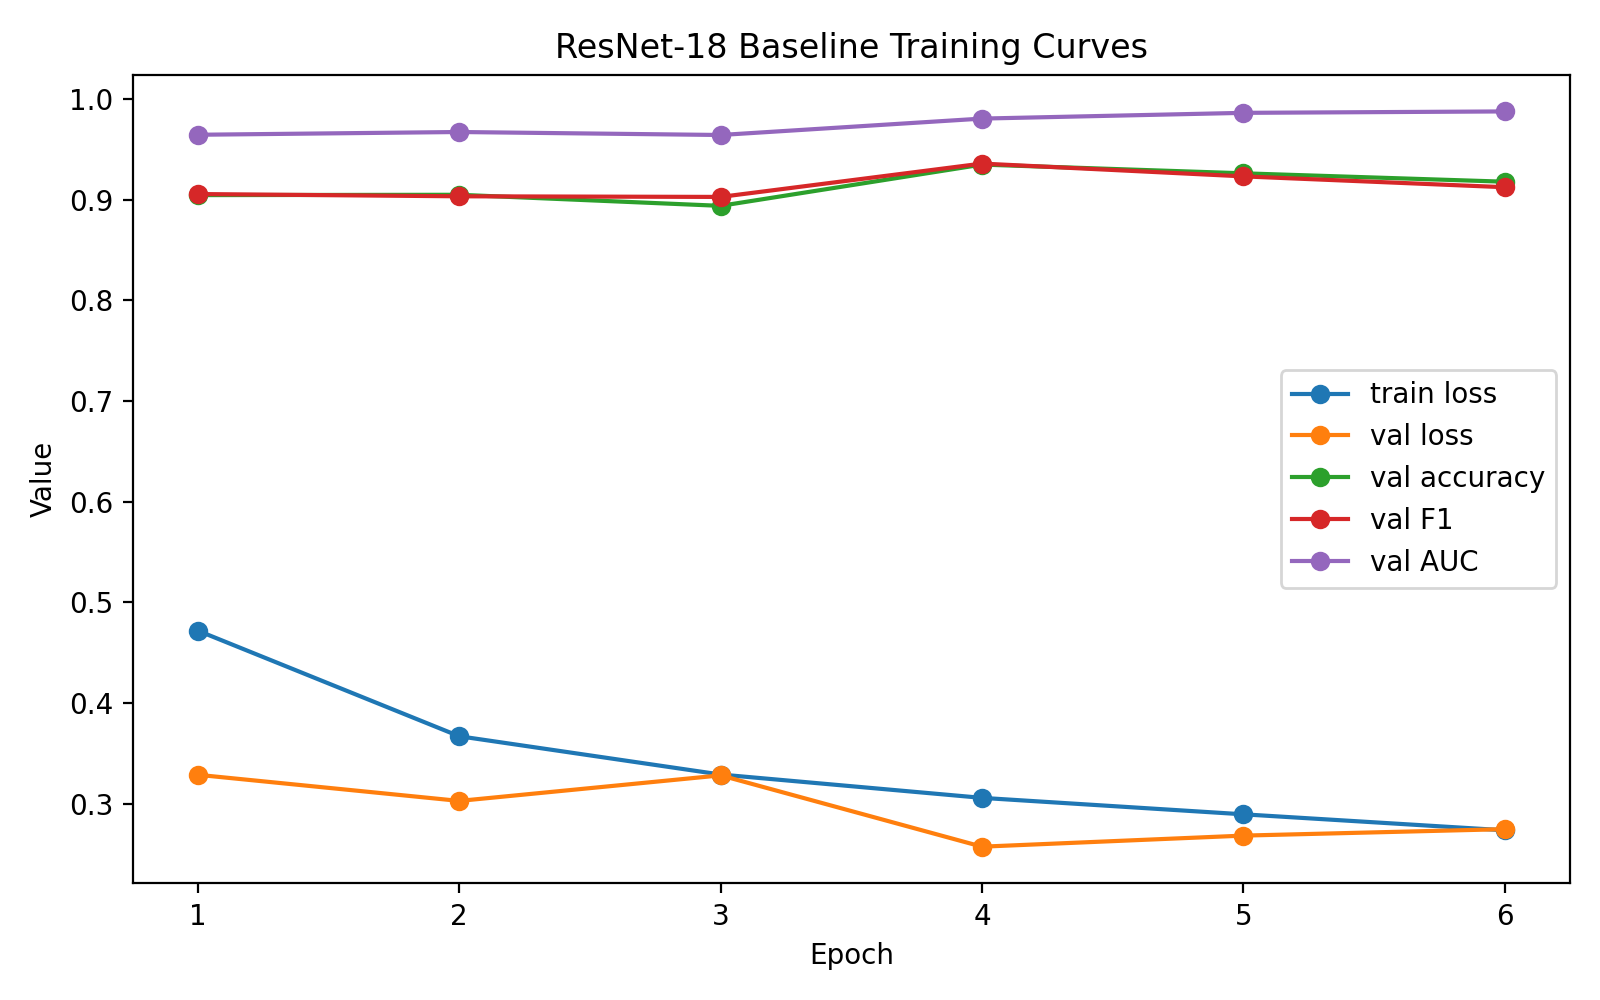
\includegraphics[width=0.95\columnwidth]{figures/step1b_resnet_training_curves.png}
    \caption{Step 1b ResNet training curves: MidJourney $\rightarrow$ SD3.}
    \label{fig:step1b_resnet_curves}
\end{figure}

\begin{figure}[H]
    \centering
    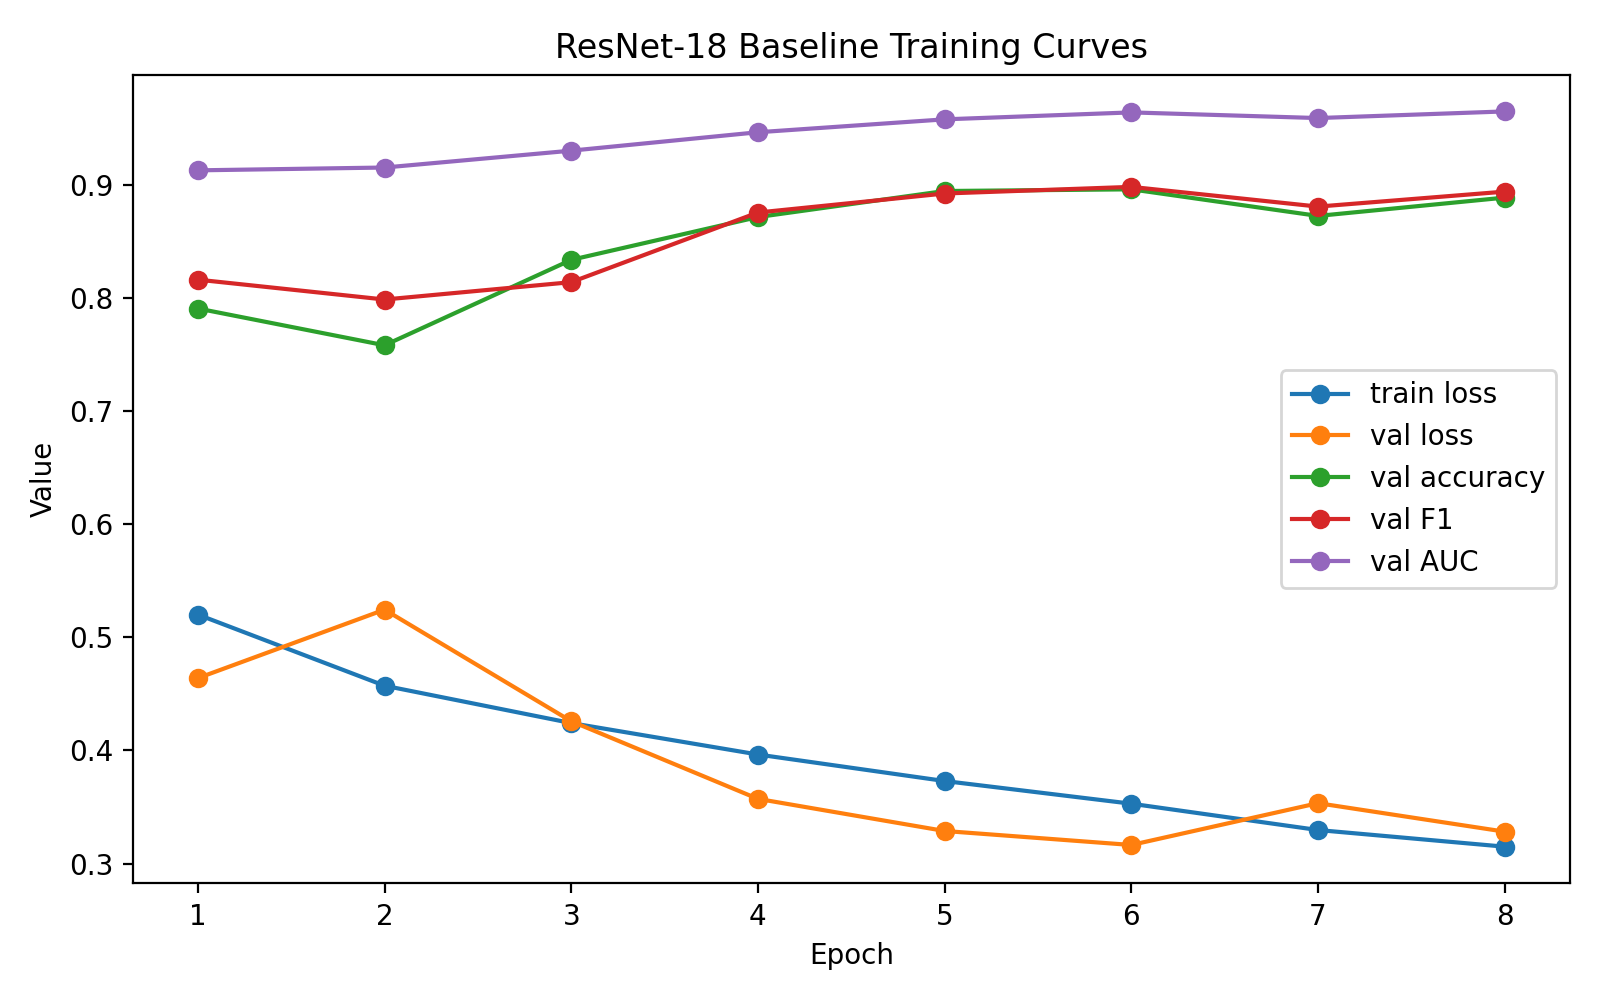
\includegraphics[width=0.95\columnwidth]{figures/step2_resnet_training_curves.png}
    \caption{Step 2 ResNet training curves: SD3+SDXL $\rightarrow$ MidJourney.}
    \label{fig:step2_resnet_curves}
\end{figure}

\begin{table}[t]
    \centering
    \caption{Unseen-generator performance. Step 1 and Step 2 use ResNet; Step 3
    repeats the same protocols with frozen CLIP features.}
    \label{tab:main_results}
    \resizebox{\columnwidth}{!}{
    \begin{tabular}{lcccc}
        \toprule
        Protocol & ResNet AUC & CLIP AUC & ResNet F1 & CLIP F1 \\
        \midrule
        SD3 $\rightarrow$ MidJourney & 0.5318 & \textbf{0.8719} & 0.1747 & \textbf{0.6633} \\
        MidJourney $\rightarrow$ SD3 & 0.5482 & \textbf{0.9153} & 0.1673 & \textbf{0.6045} \\
        SD3+SDXL $\rightarrow$ MidJourney & 0.6694 & \textbf{0.9018} & 0.3695 & \textbf{0.7096} \\
        \bottomrule
    \end{tabular}
    }
\end{table}

Figures~\ref{fig:step1a_resnet_curves}--\ref{fig:step2_resnet_curves} and
Table~\ref{tab:main_results} show that single-generator ResNet training does
not generalize well. The unseen AUC is 0.5318 for SD3 $\rightarrow$ MidJourney
and 0.5482 for MidJourney $\rightarrow$ SD3, close to random ranking. The
corresponding F1 scores, 0.1747 and 0.1673, are even more concerning: the
detector misses most fake images from the unseen generator. This indicates that
the CNN has learned source-generator cues rather than generator-invariant
evidence of synthesis.

Step 2 then adds SDXL to the SD3 training set. This raises ResNet unseen
MidJourney AUC from 0.5318 to 0.6694 and F1 from 0.1747 to 0.3695. Therefore,
generator diversity does help, but the improvement is limited. The detector is
better than the single-generator version, yet it still fails to reach a level
that would be reliable under practical generator shift.

\FloatBarrier

\subsection{Step 3: CLIP Comparison}

Step 3 is motivated by the limitation of the previous two stages. If a CNN
trained from zero overfits to generator-specific artifacts, then the next
question is whether a broader pretrained representation can provide more
transferable features. CLIP is suitable for this role because its visual encoder
is pretrained on large-scale image-text pairs. The model is encouraged to align
images with textual concepts, so its image features encode higher-level
semantic and structural information in addition to local appearance. In this
project, CLIP is not fine-tuned; only a small linear classifier is trained on
top of frozen CLIP image embeddings.

\begin{figure}[H]
    \centering
    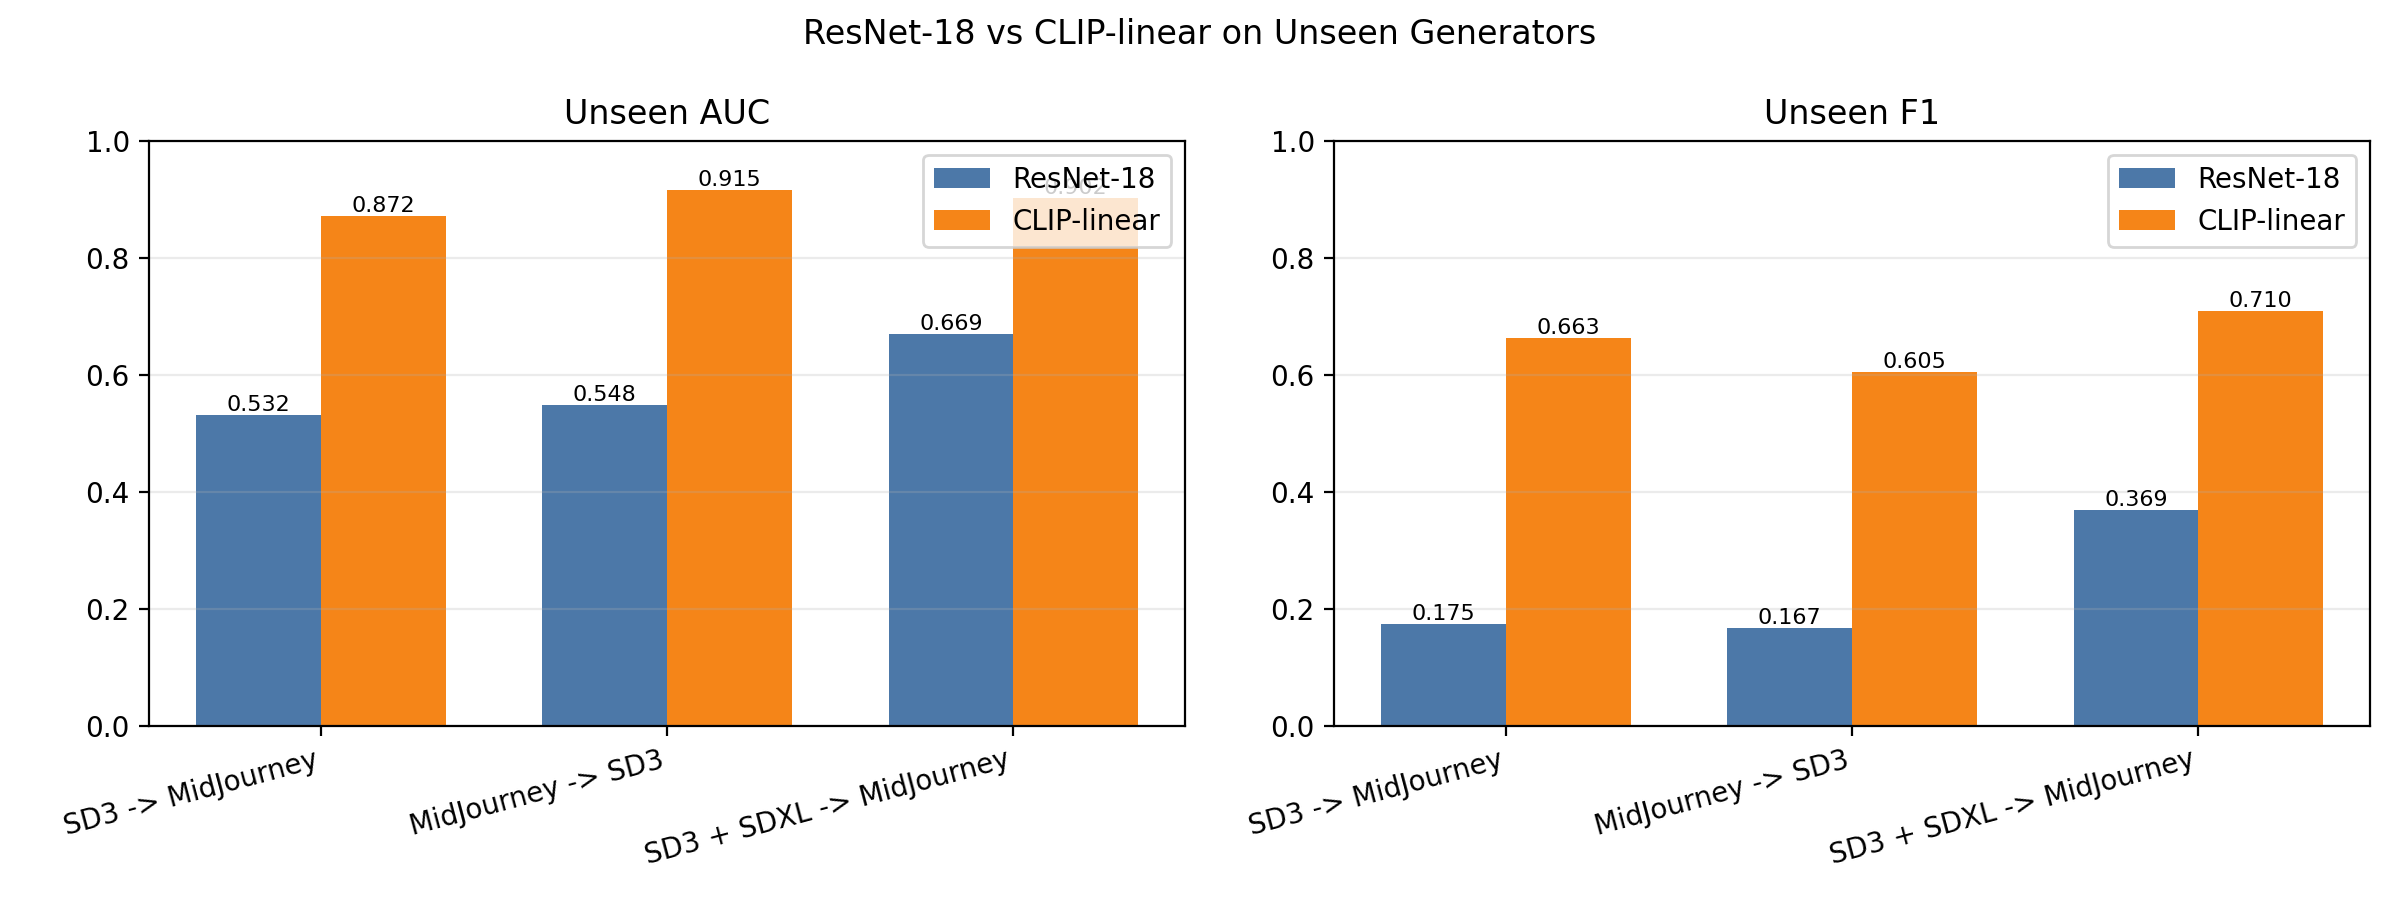
\includegraphics[width=\columnwidth]{figures/step3_clip_vs_resnet_unseen.png}
    \caption{Step 3 comparison on unseen generators. CLIP-linear improves AUC
    and F1 in all three protocols.}
    \label{fig:clip_vs_resnet}
\end{figure}

\begin{figure}[H]
    \centering
    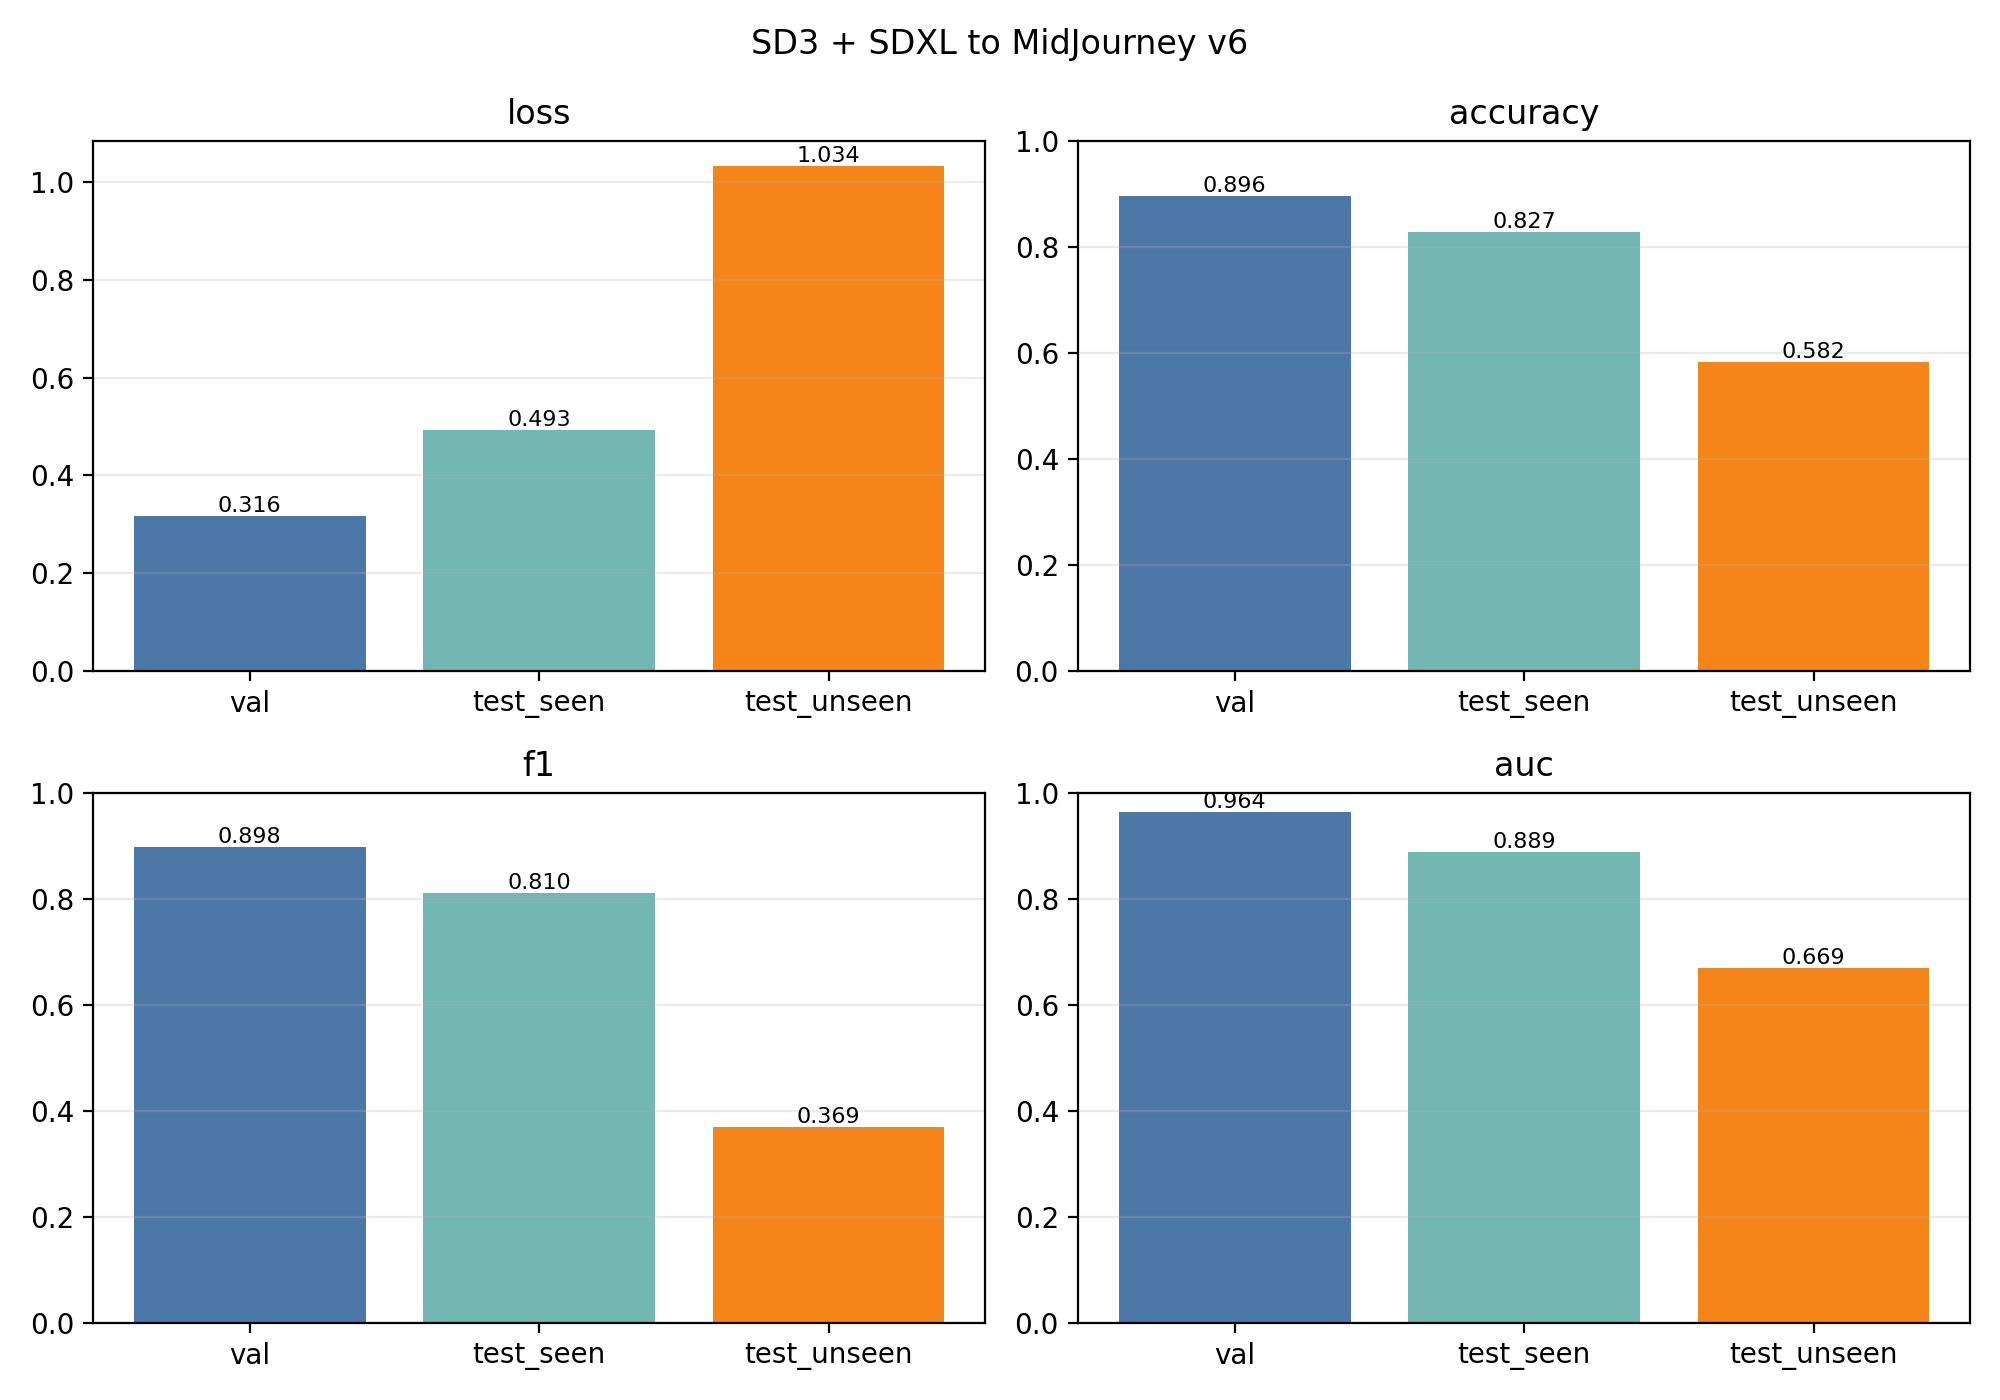
\includegraphics[width=0.95\columnwidth]{figures/step2_resnet_split_metrics.png}
    \caption{Step 2 ResNet split metrics for SD3+SDXL $\rightarrow$ MidJourney.}
    \label{fig:step2_resnet_split}
\end{figure}

\begin{figure}[H]
    \centering
    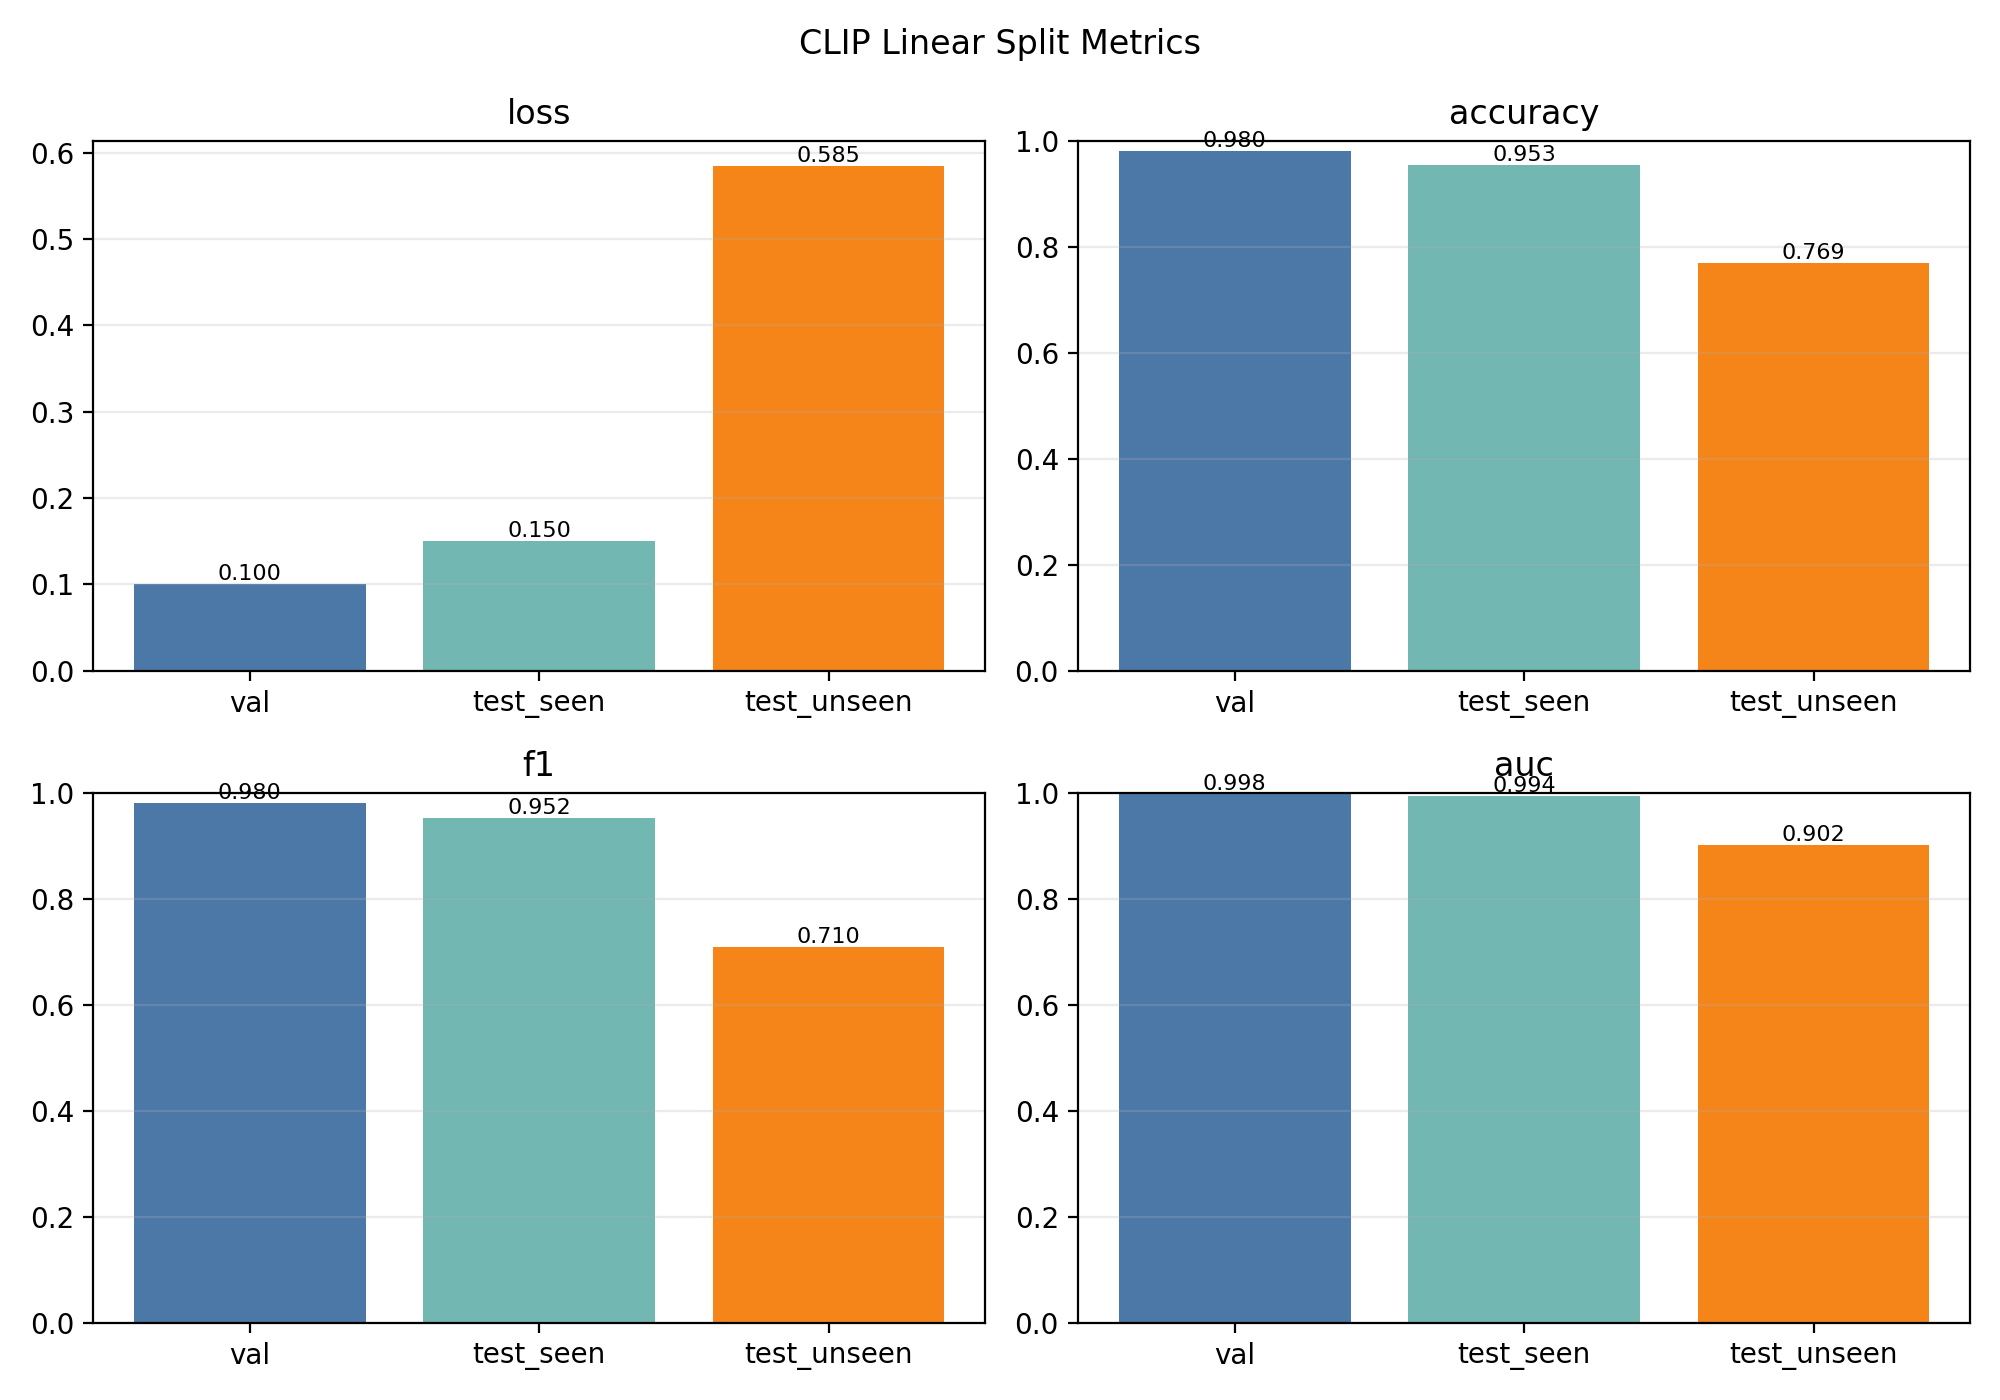
\includegraphics[width=0.95\columnwidth]{figures/step3_clip_split_metrics.png}
    \caption{Step 3 CLIP-linear split metrics across the three protocols.}
    \label{fig:step3_clip_split}
\end{figure}

\begin{figure}[H]
    \centering
    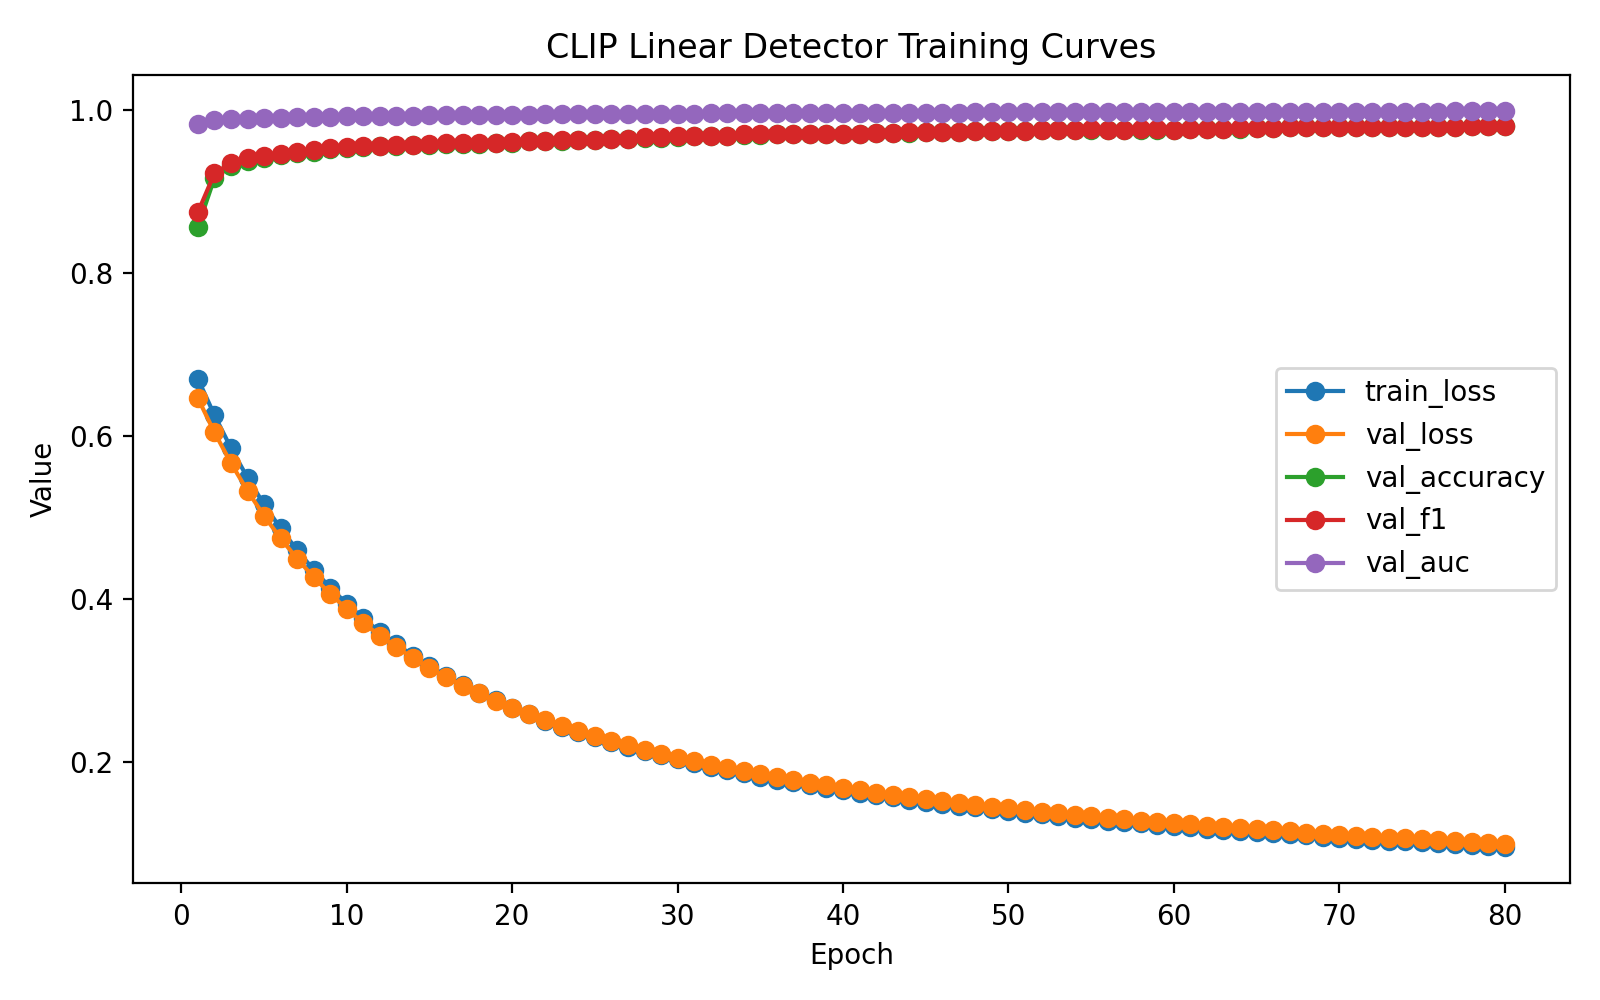
\includegraphics[width=\columnwidth]{figures/step3_clip_training_curves.png}
    \caption{Step 3 CLIP-linear training curves for SD3+SDXL $\rightarrow$
    MidJourney. The linear head converges smoothly on frozen CLIP features.}
    \label{fig:clip_curves}
\end{figure}

The difference is substantial. For SD3 $\rightarrow$ MidJourney, CLIP improves
unseen AUC from 0.5318 to 0.8719 and F1 from 0.1747 to 0.6633. For the reverse
direction, AUC increases from 0.5482 to 0.9153. In the strongest setting,
SD3+SDXL $\rightarrow$ MidJourney, CLIP reaches unseen AUC 0.9018 and F1
0.7096. Figures~\ref{fig:step2_resnet_split} and~\ref{fig:step3_clip_split}
make the improvement more direct: the ResNet split metrics still show a large
gap between seen and unseen performance, while CLIP produces a more balanced
pattern across splits.

\begin{table}[h]
\centering
\caption{Unseen-test confusion counts. Fake is the positive class.}
\label{tab:confusion}
\begin{tabular}{llrrrr}
\toprule
Method & Protocol & TN & FP & FN & TP \\
\midrule
ResNet & SD3 $\rightarrow$ MJ & 6984 & 516 & 6733 & 767 \\
ResNet & MJ $\rightarrow$ SD3 & 6323 & 1177 & 6708 & 792 \\
ResNet & SD3+SDXL $\rightarrow$ MJ & 6893 & 607 & 5663 & 1837 \\
CLIP & SD3 $\rightarrow$ MJ & 7249 & 251 & 3654 & 3846 \\
CLIP & MJ $\rightarrow$ SD3 & 7343 & 157 & 4183 & 3317 \\
CLIP & SD3+SDXL $\rightarrow$ MJ & 7315 & 185 & 3274 & 4226 \\
\bottomrule
\end{tabular}
\end{table}

Table~\ref{tab:confusion} makes the error pattern more concrete. In the
SD3-to-MidJourney protocol, ResNet detects only 767 of 7500 fake MidJourney
images, while CLIP detects 3846. In the multi-generator protocol, ResNet
improves to 1837 true positives, but CLIP still more than doubles that number
to 4226 while keeping false positives low. The main gain is therefore not only
better ranking AUC; CLIP also reduces the number of fake images that are
mistakenly accepted as real.

\FloatBarrier

\subsection{Qualitative Examples}

\begin{figure}[H]
    \centering
    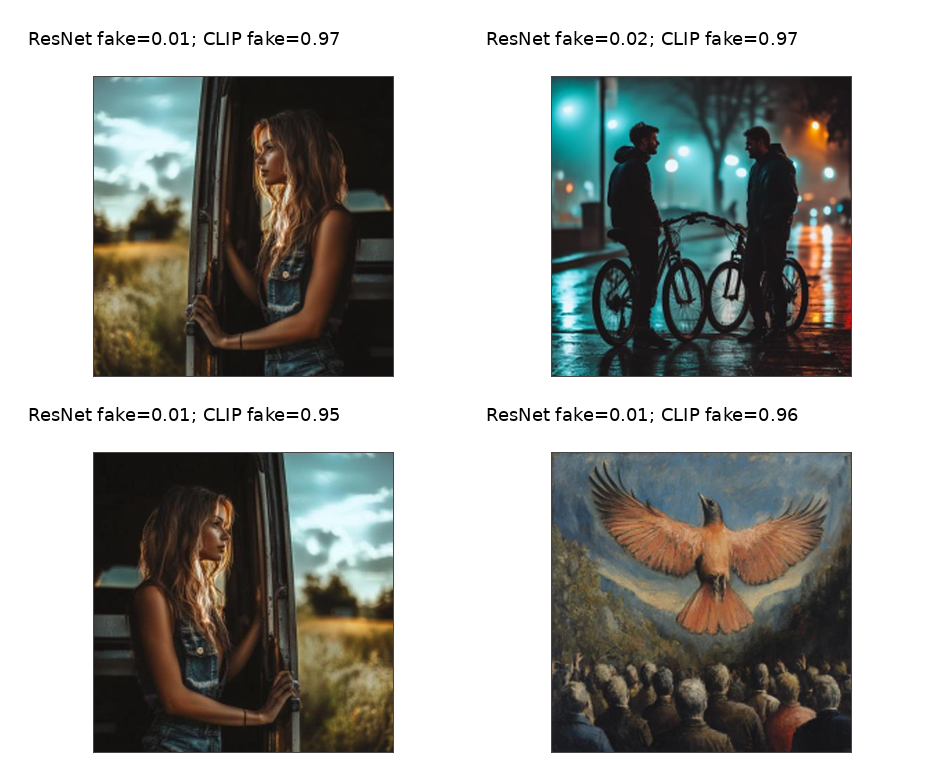
\includegraphics[width=0.95\columnwidth]{figures/qual_resnet_missed_clip_detected_2x2.png}
    \caption{Unseen MidJourney fake images missed by ResNet but detected by
    CLIP. Numbers are predicted fake probabilities.}
    \label{fig:qualitative}
\end{figure}

Figure~\ref{fig:qualitative} shows fake MidJourney images from the unseen split
where ResNet predicts ``real'' but CLIP predicts ``fake''. These examples make
the numerical result more interpretable. ResNet appears sensitive to whether
the target generator shares the same low-level artifacts as the training
generator. CLIP, by contrast, can use broader cues such as object coherence,
scene composition, and semantic plausibility. This does not mean CLIP is a
perfect detector, but it explains why frozen CLIP features are more robust than
a CNN trained only on the available synthetic sources.

\subsection{Limitations}

This study evaluates a focused subset of MS COCOAI protocols rather than all
generator combinations. CLIP is used as a frozen encoder only, so the results
do not test whether end-to-end fine-tuning would further improve performance.
The qualitative analysis is also limited to a small number of examples. Another
limitation is that this project uses image-level binary labels only. It does
not localize manipulated regions or explain decisions with saliency maps, so
the current detector is best interpreted as a classification baseline rather
than a forensic explanation system.

\section{Conclusion}

This project studied AI-generated image detection under cross-generator
distribution shift. ResNet-18 performs reasonably on seen generators but fails
to robustly detect unseen generators. Multi-generator training improves
generalization, and frozen CLIP features produce the strongest results across
all protocols. Future work should evaluate additional generator combinations,
frequency-domain features, and CLIP fine-tuning.

\bibliographystyle{IEEEtran}
\balance
\bibliography{references}

\clearpage
\appendices

\section{Detailed Experimental Configuration}

\begin{table}[h]
    \centering
    \caption{Curated split sizes used in each protocol.}
    \resizebox{\columnwidth}{!}{
    \begin{tabular}{lrrrr}
        \toprule
        Protocol & Train & Val & Seen test & Unseen test \\
        \midrule
        SD3 $\rightarrow$ MidJourney & 14000 & 3000 & 15000 & 15000 \\
        MidJourney $\rightarrow$ SD3 & 14000 & 3000 & 15000 & 15000 \\
        SD3+SDXL $\rightarrow$ MidJourney & 28000 & 6000 & 30000 & 15000 \\
        \bottomrule
    \end{tabular}
    }
\end{table}

\begin{table}[h]
    \centering
    \caption{Main hyperparameter settings.}
    \resizebox{\columnwidth}{!}{
    \begin{tabular}{lll}
        \toprule
        Setting & ResNet-18 & CLIP-linear \\
        \midrule
        Backbone & ResNet-18 from scratch & frozen CLIP ViT-B/32 \\
        Input size & 224$\times$224 & CLIP processor default \\
        Optimizer & AdamW & AdamW \\
        Learning rate & $10^{-4}$ & $10^{-3}$ \\
        Weight decay & $10^{-3}$ & $10^{-4}$ \\
        Batch size & 128 & 256 feature extraction \\
        Early stopping & val loss, patience 2 & val loss, patience 8 \\
        Trainable head & two-class FC layer & linear real/fake head \\
        \bottomrule
    \end{tabular}
    }
\end{table}

\section{Implementation Notes}

The ResNet baseline uses a two-class cross-entropy objective. The final fully
connected layer is replaced with a real/fake head. The CLIP detector extracts
normalized image embeddings once and caches them as NumPy arrays. A linear
classifier is then trained on top of the frozen embeddings. This design keeps
the CLIP experiment lightweight and makes the comparison focus on feature
quality rather than full-model fine-tuning.

\section{Code Archive and Reproducibility Commands}

The complete project code is archived at:
\begin{center}
\url{https://github.com/Obl1vion31/aigc-detect}
\end{center}
The appendix therefore does not duplicate the full source code. Instead, it
records the role of each script and the commands needed to reproduce the main
experiments. The experiments are organized under \texttt{outputs/current}. The
main scripts are:
\begin{itemize}
    \item \texttt{curate\_mscocoai\_split.py}: reads MS COCOAI parquet files,
    filters selected generators, and writes curated train/validation/test
    splits.
    \item \texttt{train\_resnet18\_baseline.py}: trains the ResNet-18 baseline
    from scratch and evaluates seen and unseen generator splits.
    \item \texttt{train\_clip\_linear\_detector.py}: extracts frozen CLIP image
    features, caches them, and trains a linear real/fake classifier.
\end{itemize}

The following command pattern illustrates the three experiment types. In the
actual runs, \texttt{TRAIN\_GENS} is replaced by \texttt{stable\_diffusion\_3},
\texttt{midjourney\_v6}, or \texttt{stable\_diffusion\_3,sdxl}; \texttt{UNSEEN}
is the held-out generator.
\begin{verbatim}
python curate_mscocoai_split.py
  --train-generators TRAIN_GENS
  --unseen-generators UNSEEN

python train_resnet18_baseline.py
  --data-dir CURATED_SPLIT

python train_clip_linear_detector.py
  --data-dir CURATED_SPLIT
\end{verbatim}

\section{Qualitative Example Selection}

The qualitative examples in the main paper are selected from fake MidJourney
images in the unseen split of the SD3 to MidJourney protocol. They satisfy:
\begin{equation}
P_{\mathrm{ResNet}}(\mathrm{fake}) < 0.5,\quad
P_{\mathrm{CLIP}}(\mathrm{fake}) \geq 0.5.
\end{equation}
Thus, each example is a ResNet false negative but a CLIP true positive. This
selection rule is used to show the specific error type reduced by CLIP: fake
images that a source-trained CNN would incorrectly accept as real.

\section{Core Pseudocode}

This section summarizes the key computation without reproducing the full code.
The CLIP detector freezes the encoder and trains only a linear head:
\begin{verbatim}
z = clip_image_encoder(x)
z = normalize(z)
logits = linear_head(z)
loss = cross_entropy(logits, y)
\end{verbatim}

The ResNet baseline trains the classifier end-to-end:
\begin{verbatim}
logits = resnet18(x)
loss = cross_entropy(logits, y)
loss.backward()
optimizer.step()
\end{verbatim}

\end{document}
